\section{Graph des Stromnetzmodells}

Die Visualisierung eines gesamten Stromnetzwerkes auf einem kleinen Computerbildschirm ist nicht ganz so trivial, wie die Auflistung der aktuellen Fehler im Netzmodell. Dank der Bibliothek Cytoscape ist die Implementierung eines Graphen in einer Webanwendung erheblich leichter. Dennoch haben wir uns viele Gedanken machen müssen, wie wir diesen Teil des Prototypen gestalten wollen.

Die grundlegende Frage bei der Visualisierung von diesen spezifischen Daten ist: Sollen die relevanten Informationen im Graph als Knoten oder Kanten abgebildet werden? Standardmäßig geht ein Benutzer davon aus, dass die Knoten mehr Relevanz haben, als die Kanten, da letztere nur das Verbindungsstück zwischen den wesentlichen Elementen darstellen. Doch in manchen Szenarien, wie bei einem Stromnetzwerk zum Beispiel, können die Informationen auch in den Kanten enthalten sein. Immerhin ist fast jedes Element in unseren Daten nur mit exakt zwei Endpunkten verknüpft. Das ruft förmlich nach den Eigenschaften der Kanten.

Nichtdestotrotz haben Clemens und Felix sich dazu entschieden, die Elemente des Stromnetzwerkes einfach zu Knoten heraufzustufen, da dieser Ansatz viel intuitiver für die Ingenieure von Siemens ist. Aus diesem Grund haben die meisten Knoten in Abbildung \ref{fig:AngularGraphPrototype} auch nur zwei anliegende Kanten zu anderen Knoten. 

Ein weiterer Vorteil der Darstellung der Elemente in den Knoten des Graphen ist die erleichterte Visualisierung der Namen dieser Modellobjekte sowie intuivtivere Interaktionsmöglichkeiten mit dem Benutzer. Denn viele Benutzer wissen, dass Knoten in einem Graphen auswählbar sind, während die Selektion einer Kante eher befremdlich wirkt.

\begin{figure}
    \centering
    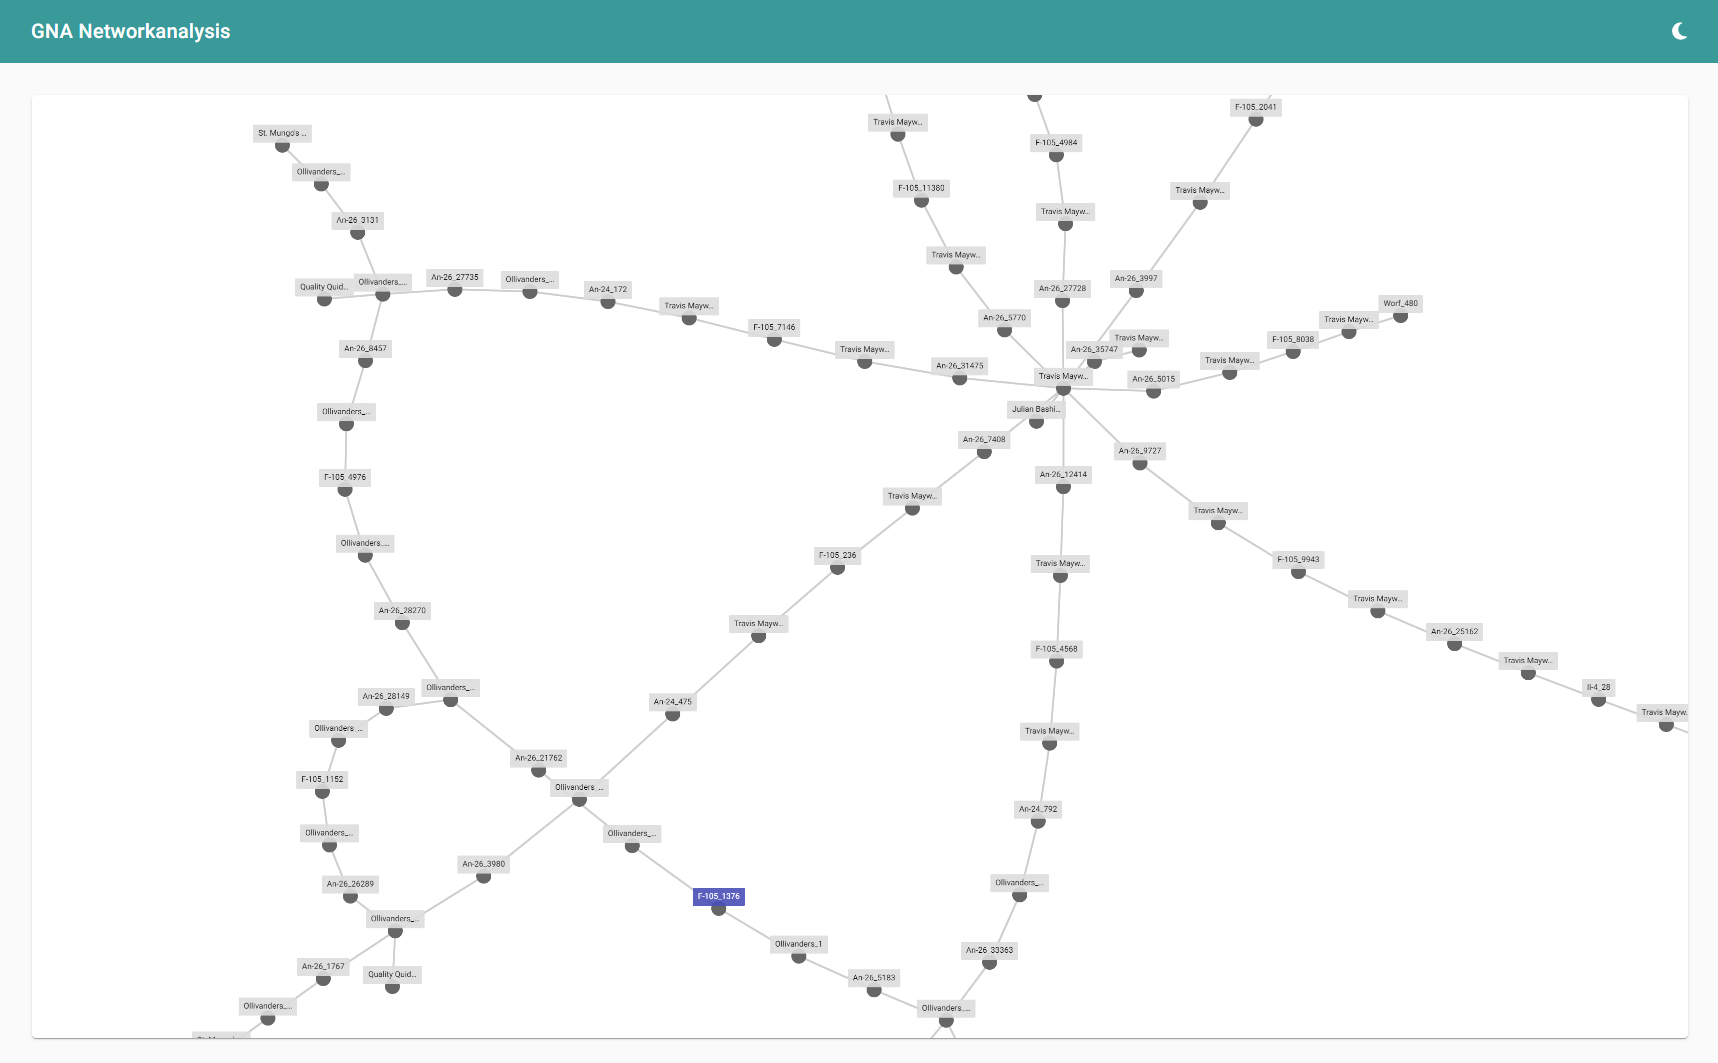
\includegraphics[width=1\textwidth]{content/img/Empire/Frontend/Angular_Graph_Prototype.png}
    \caption{Visualisierung eines Teils des Stromnetzwerkes in einem Graphen}
    \label{fig:AngularGraphPrototype}
\end{figure}
\FloatBarrier

Eine weitere Überlegung dieser Visualisierungsmethode ist der Einstiegspunkt beziehungsweise der Knoten, welcher als erstes geladen wird, gewesen. Denn aufgrund der schieren Menge an Elementen im Stromnetzwerk ist es einfach unmöglich alle Daten auf einmal zu laden. Aus diesem Grund wird immer nur ein Stück beziehungsweise ein kleiner Teil des Stromnetzwerkes angezeigt. Dabei ergibt sich jedoch die Frage: Welcher Teil des Netzwerks soll angezeigt werden, wenn nicht das gesamte Netzwerk angezeigt werden kann? Anders formuliert benötigen wir ein Startelement, von welchem aus die weiteren angeschlossenen Elemente geladen werden können. Somit haben wir die Möglichkeit, das Laden der Elemente auf eine gewisse Tiefe zu reduzieren. Folgendermaßen wird automatisch nur ein Teil des Graphen geladen, was wiederum die Schnelligkeit der Visualisierung deutlich erhöht.

Aus diesen genannten Gründen ist es bei unserer Applikation nicht möglich, den Graph ohne Startelement zu visualisieren. Und genau deswegen können Sie den Graphen auch nur ansehen, wenn Sie auf den \wordindoublequotes{Go to Graph →}-Button bei der Fehlertabelle klicken. Denn somit haben wir sichergestellt, dass der Graph mit einem fehlerhaften Objekt im Netzmodell startet, dessen nähere Umgebung Sie angenehm analysieren können. In Abbildung \ref{fig:AngularGraphCurrentErrorPrototype} können Sie sehr gut erkennen, dass das Startelement im Graphen auch blau markiert ist, damit die Siemens Ingenieure effizient und effektiv den Ursprung des Fehlers im Netzmodell ausfindig machen können.

\begin{figure}
    \centering
    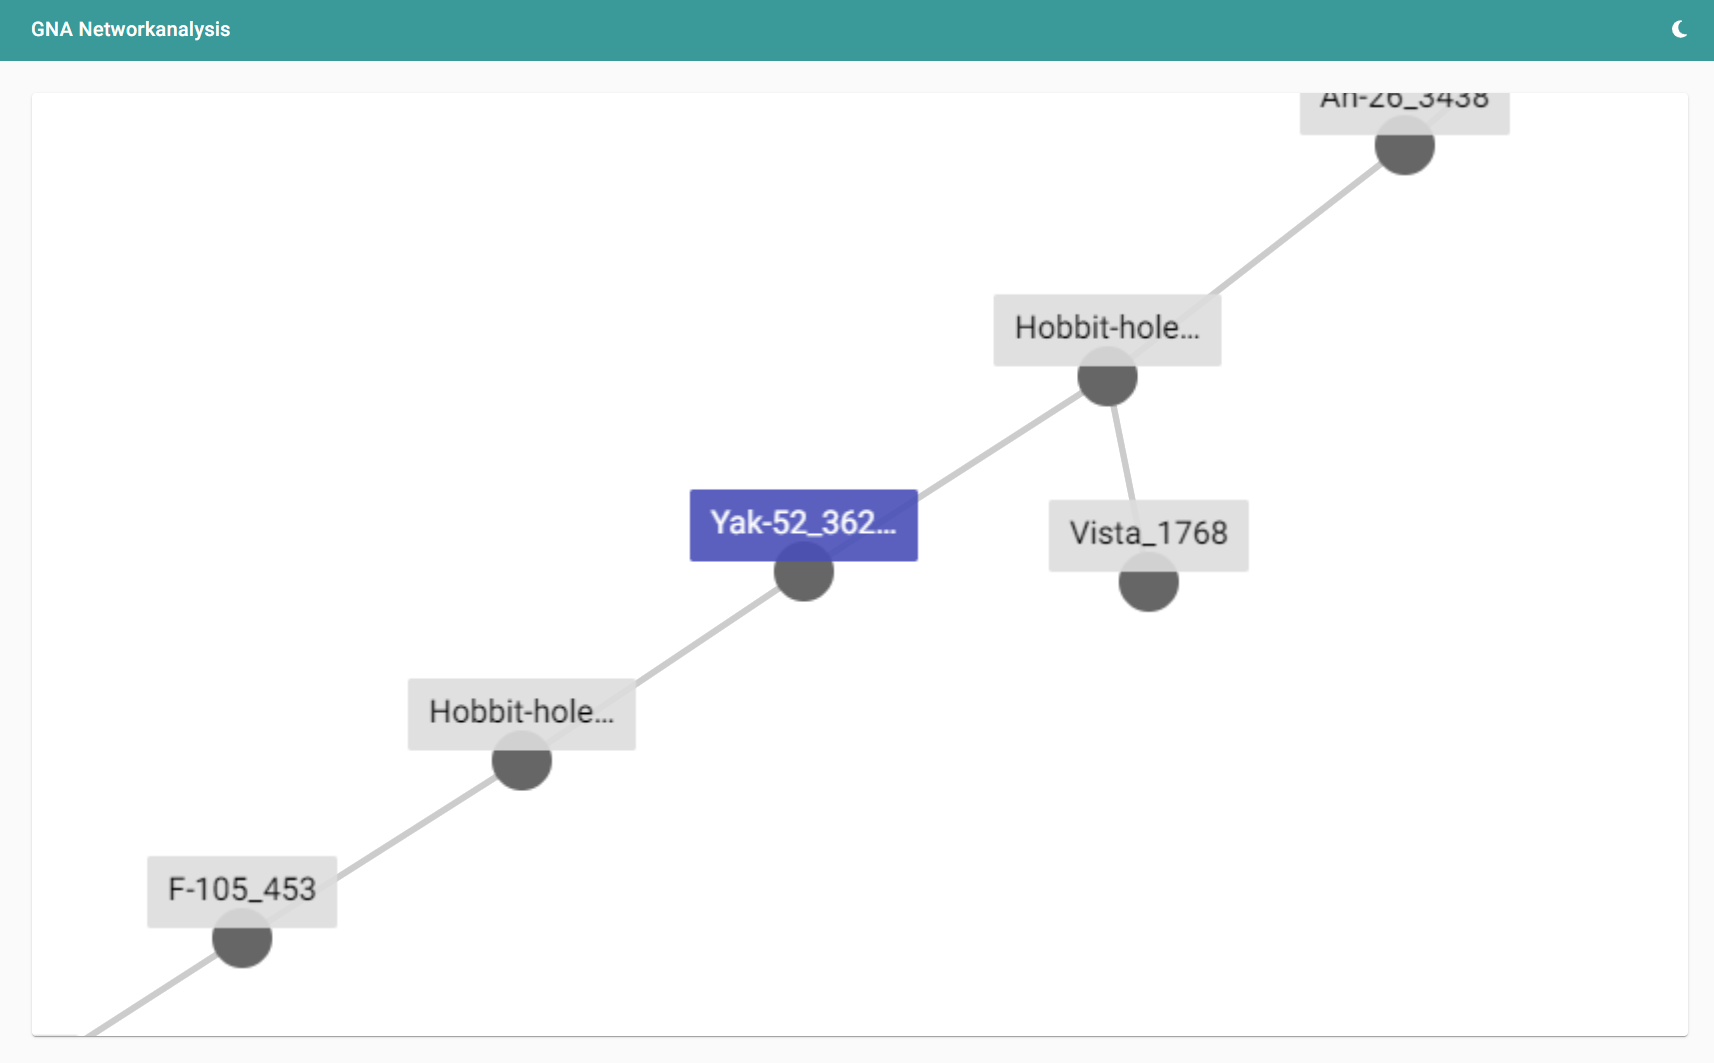
\includegraphics[width=1\textwidth]{content/img/Empire/Frontend/Angular_Graph_Current_Error_Prototype.png}
    \caption{Aktuelles fehlerhaftes Netzmodellobjekt im Graphen blau markiert}
    \label{fig:AngularGraphCurrentErrorPrototype}
\end{figure}
\FloatBarrier

In dieser Abbildung (\ref{fig:AngularGraphCurrentErrorPrototype}) sehen Sie auch trotz Anonymisierung der Daten, dass zwischen zwei aktiven Elementen (Schalter, Transformatoren, Widerstände, Generatoren, Sicherungen, usw.) meistens ein passives Element (hauptsächlich Leiter) liegt. Aktive Elemente beschreiben in dem Kontext eher Elemente, welche Eigenschaften des Stroms verändern, während passive diesen nur transportieren. Wie Sie sehen können, kommen diese beiden Gruppen -- aktive und passive Elemente -- abwechselnd hintereinander im Netzmodell vor: \wordindoublequotes{Hobbit-hole} -- \wordindoublequotes{Yak-52} -- \wordindoublequotes{Hobbit-hole}. Noch besser ist diese besondere Eigenschaft im Abbildung \ref{fig:AngularGraphAlternatingElementsPrototype} zu erkennen, wo sich \wordindoublequotes{Yak} und \wordindoublequotes{Dori} alternierend entlang der gelb markieren Verbindung ergänzen.

\setcapindent{90pt}
\begin{figure}
    \centering
    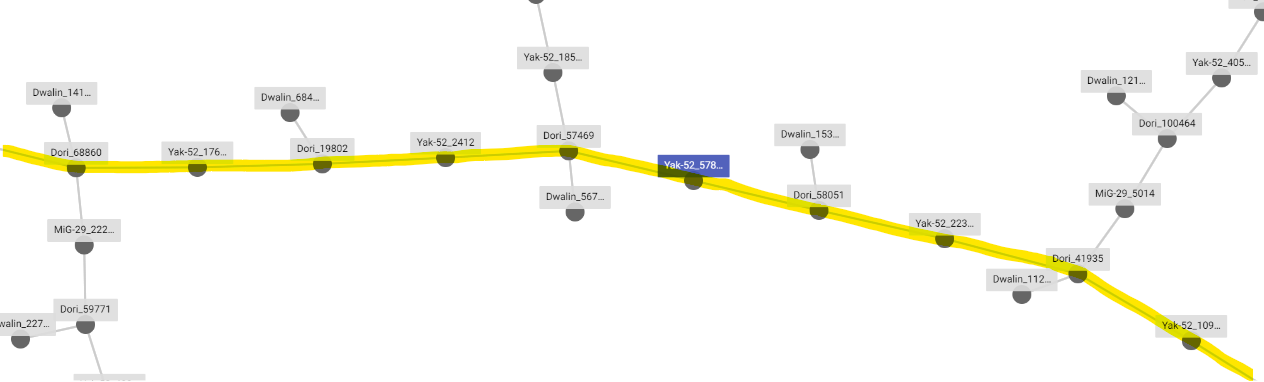
\includegraphics[width=1\textwidth]{content/img/Empire/Frontend/Angular_Graph_Alternating_Elements_Prototype.png}
    \caption{Abwechselnde Vorkommnis der verschiedenen Elementgruppen im Stromnetzwerk}
    \label{fig:AngularGraphAlternatingElementsPrototype}
\end{figure}
\FloatBarrier

Im Sinne des Graphen ist auch anzumerken, dass die Positionierung der Knoten keine geografische Bedeutung haben, da uns diese Art von topografischen Daten nicht zur Verfügung steht. Stattdessen werden die Knoten mithilfe des \emph{cola}-Layouts möglichst effizient angeordnet. Effizienz in diesem Sinne bedeutet, dass sich die Knoten, wären sie Atome, in einer möglichst ruhigen, entspannten Position und angenehmen Entfernung von anderen Knoten befinden. Dieses Layout unterstützt dementsprechend die Darstellung eines natürlichen biologischen Systems, da sich beispielsweise auch Zellen im menschlichen Körper gleichmäßig in den Blutbahnen verteilen. 